\section{Use-case Diagrams}
\subsection{Use-case Diagram for the Whole System}
\begin{figure}[htbp]
	\centering
	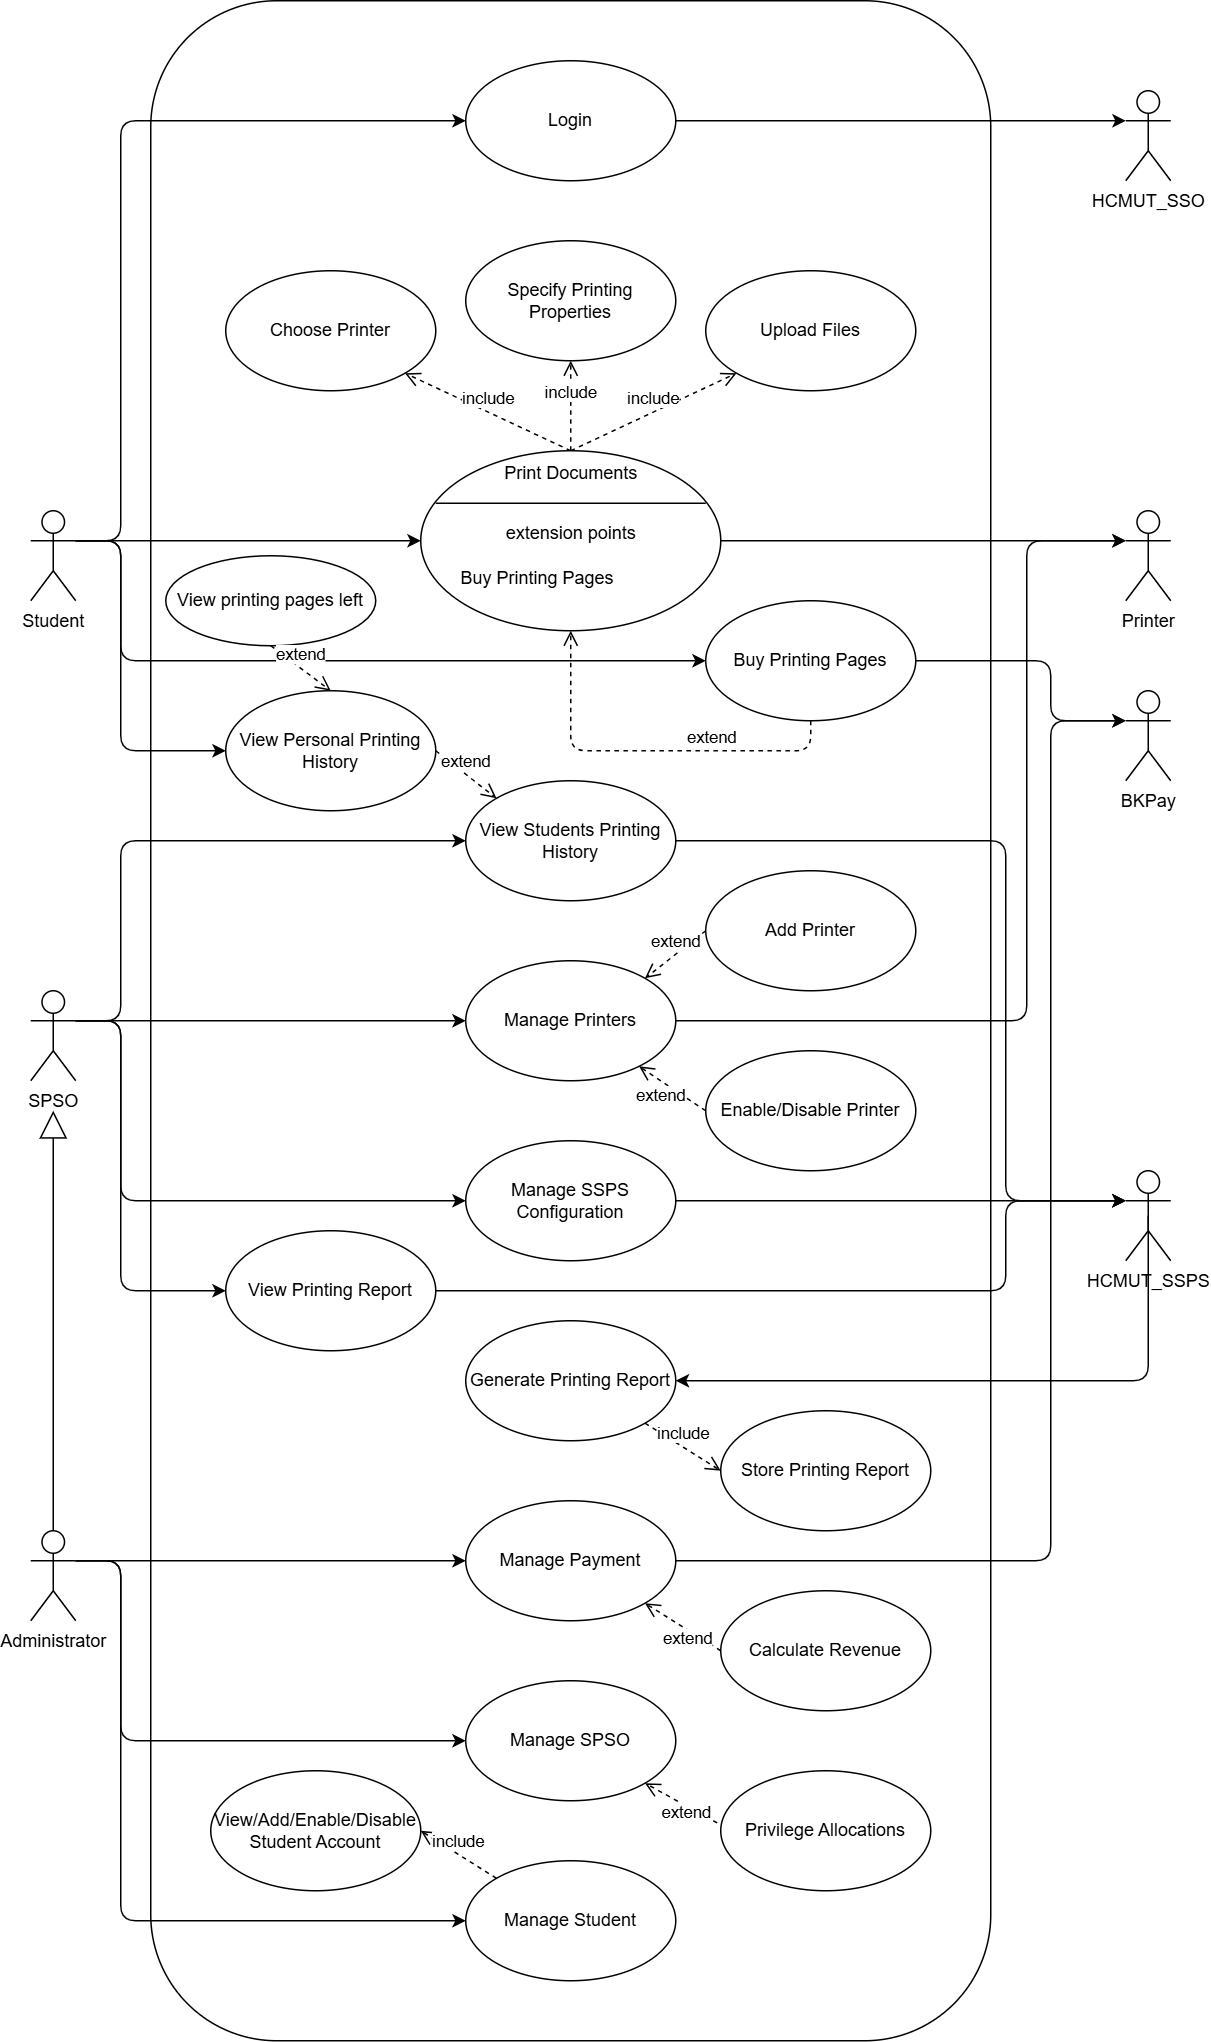
\includegraphics[width=0.62\textwidth]{Images/Usecases/System_usecase.png}
	\caption{\fontsize{12pt}{0pt}\selectfont System Usecase}
\end{figure}
\newpage


\subsection{Use-case Diagram}
\subsubsection{Printing Module}
\begin{figure}[htbp]
	\centering
	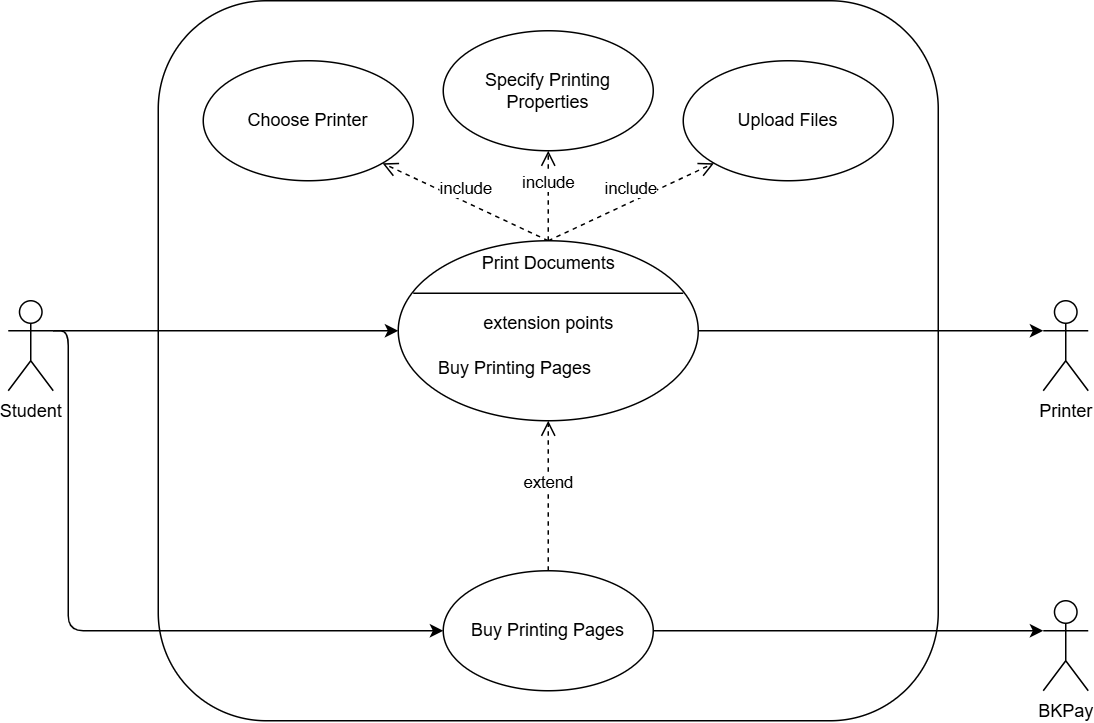
\includegraphics[width=1.0\textwidth]{Images/Usecases/Print_usecase.png}
	\vspace{15pt}
	\caption{\fontsize{12pt}{0pt}\selectfont Printing Usecase}
\end{figure}
\newpage

\subsubsection{Login Module}
\begin{figure}[htbp]
	\centering
	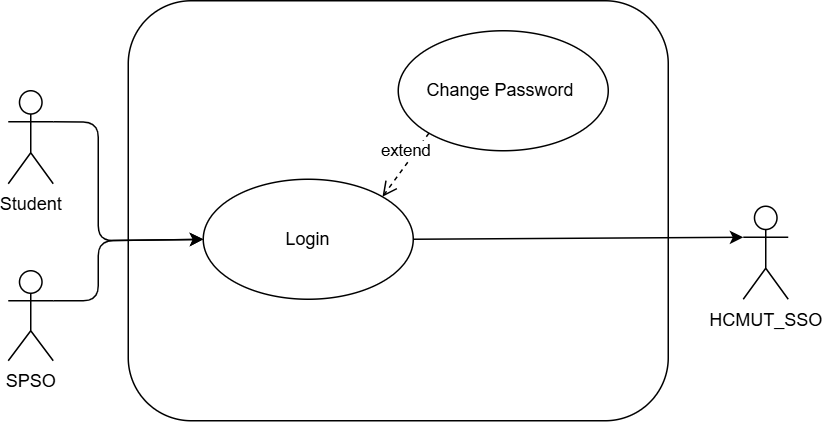
\includegraphics[width=1.0\textwidth]{Images/Usecases/Login_usecase.png}
	\vspace{15pt}
	\caption{\fontsize{12pt}{0pt}\selectfont Login Usecase}
\end{figure}
\newpage

\subsubsection{Printer Management Module}
\begin{figure}[htbp]
	\centering
	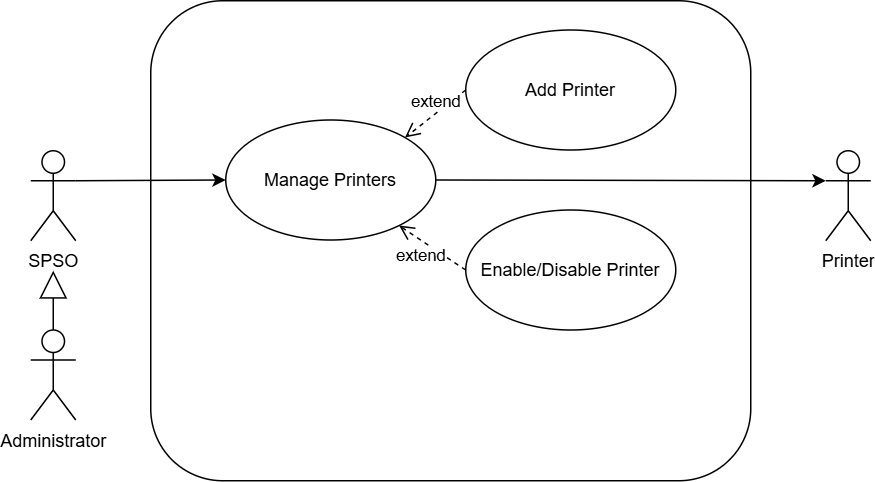
\includegraphics[width=1.0\textwidth]{Images/Usecases/Printer_Management_usecase.png}
	\vspace{15pt}
	\caption{\fontsize{12pt}{0pt}\selectfont Printer Management Usecase}
\end{figure}
\newpage

\subsubsection{View Printing History Module}
\begin{figure}[htbp]
	\centering
	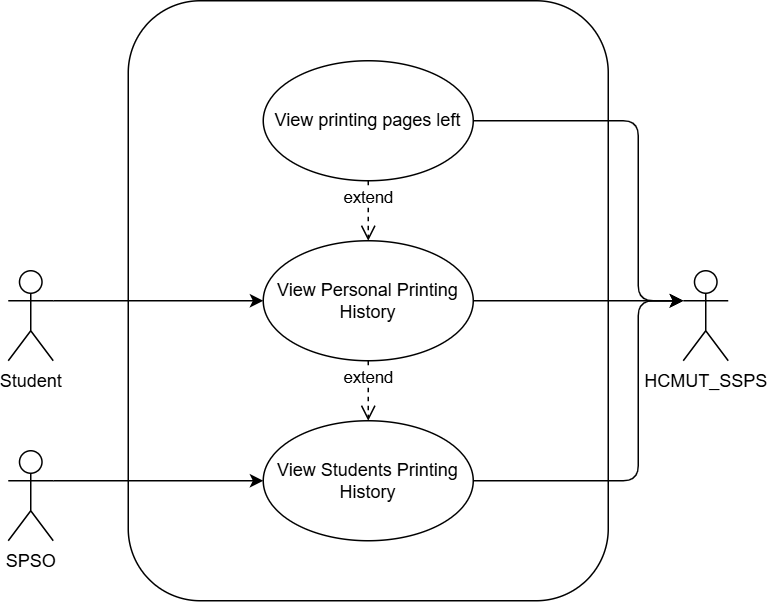
\includegraphics[width=1.0\textwidth]{Images/Usecases/Printing_History_usecase.png}
	\vspace{15pt}
	\caption{\fontsize{12pt}{0pt}\selectfont View Printing History Usecase}
\end{figure}
\newpage

\subsubsection{Generate Printing Report Module}
\begin{figure}[htbp]
	\centering
	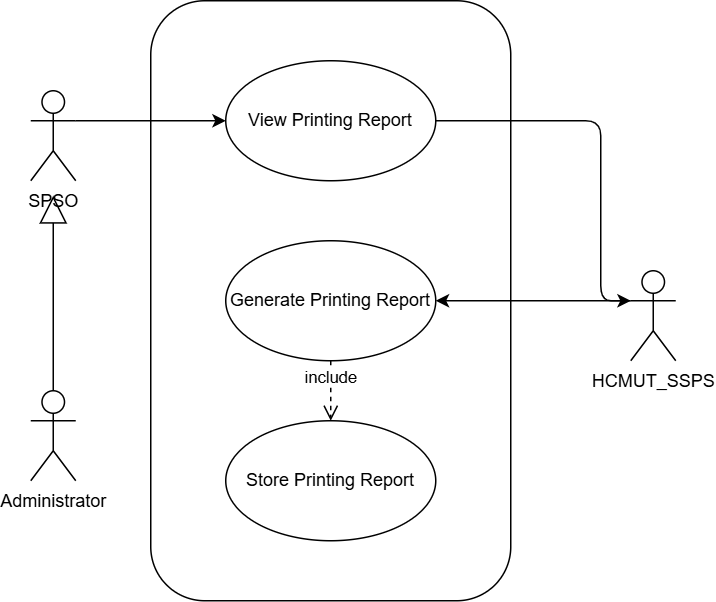
\includegraphics[width=1.0\textwidth]{Images/Usecases/View_Printing_Report_usecase.png}
	\vspace{15pt}
	\caption{\fontsize{12pt}{0pt}\selectfont Generate Printing Report Usecase}
\end{figure}
\newpage

\subsection{The Details of Usecases}
\subsubsection{Print Documents Module}
\begin{table}[h!]
	\centering
	\begin{tabular}{ |p{4cm}|p{3cm}|p{3cm}|p{3cm}|  }
		\hline
		Use Case Name:    & \multicolumn{3}{l|}{Printing Documents}                                                                                   \\
		\hline
		Actors:           & \multicolumn{3}{p{10cm}|}{Sinh viên}                                                                                      \\
		\hline
		Description:      & \multicolumn{3}{p{10cm}|}{Sinh viên tải tài liệu lên và in tài liệu bằng cách chọn máy in và thiết lập các thuộc tính in.
		Sinh viên phải mua số trang in trước khi in.}                                                                                                 \\
		\hline
		Preconditions:    & \multicolumn{3}{p{10cm}|}{Người dùng đã đăng nhập vào ứng dụng và đang sở hữu số trang có thể in nhất định.}              \\
		\hline
		Normal Flow:      & \multicolumn{3}{p{10cm}|}{
			1. Sinh viên chọn chức năng "In tài liệu" từ giao diện ứng dụng.\newline
			2. Sinh viên tải file tài liệu cần in lên hệ thống.\newline
			3. Sinh viên chọn máy in mong muốn từ danh sách các máy in có sẵn.\newline
			4. Sinh viên thiết lập các thuộc tính in (cỡ giấy, trang cần in, in một/hai mặt, số bản in, v.v).\newline
			5. Sinh viên xác nhận thông tin in và nhấn "In".\newline
			6. Máy in thực hiện lệnh in và trả lại kết quả cho sinh viên.
		}                                                                                                                                             \\
		\hline
		Exceptions:       & \multicolumn{3}{p{10cm}|}{
			Exception 1 in step 5:\newline
			1. Nếu quá trình in bị lỗi (hết giấy, kẹt giấy), hệ thống sẽ thông báo lỗi và yêu cầu sinh viên chọn máy in khác hoặc liên hệ hỗ trợ kỹ thuật.
		}                                                                                                                                             \\
		\hline
		Alternative Flow: & \multicolumn{3}{p{10cm}|}{
			Alternative 1 in step 2:\newline
			3. Nếu file tải lên không đúng định dạng, hệ thống sẽ yêu cầu sinh viên chọn file khác.\newline
			Alternative 2 in step 3:\newline
			4. Nếu không có máy in khả dụng, hệ thống sẽ thông báo cho sinh viên và yêu cầu thử lại sau.\newline
			Alternative 3 in step 2:\newline
			3. Nếu số trang cần in vượt quá số trang sinh viên có, hệ thống sẽ thông báo không hợp lệ và yêu cầu sinh viên mua thêm số trang in
			hoặc giảm số trang cần in.

		}                                                                                                                                             \\
		\hline
	\end{tabular}
\end{table}
\newpage

\subsubsection{Login Module}
\begin{table}[h!]
	\centering
	\begin{tabular}{ |p{4cm}|p{3cm}|p{3cm}|p{3cm}|  }
		\hline
		Use Case Name:    & \multicolumn{3}{l|}{Login}                                                                         \\
		\hline
		Actors:           & \multicolumn{3}{p{10cm}|}{Sinh viên, SPSO, HCMUT\_SSO}                                             \\
		\hline
		Description:      & \multicolumn{3}{p{10cm}|}{Người dùng đăng nhập và truy cập hệ thống thông qua dịch vụ HCMUT\_SSO.} \\
		\hline
		Preconditions:    & \multicolumn{3}{p{10cm}|}{
			- Người dùng có một tài khoản đã đăng ký sẵn.\newline
			- Dịch vụ xác thực HCMUT\_SSO đang hoạt động.\newline
			- Người dùng đang ở trang đăng nhập.
		}                                                                                                                      \\
		\hline
		Normal Flow:      & \multicolumn{3}{p{10cm}|}{
			1. Người dùng điều hướng đến trang đăng nhập của hệ thống.\newline
			2. Hệ thống chuyển hướng người dùng đến trang xác thực HCMUT\_SSO.\newline
			3. Người dùng nhập thông tin đăng nhập HCMUT\_SSO (tên người dùng và mật khẩu)\newline
			4. Dịch vụ HCMUT\_SSO xác minh thông tin đăng nhập và xác thực người dùng. \newline
			5. Xác thực thành công.\newline
			6. Người dùng được chuyển hướng quay lại trang chủ hoặc dashboard của hệ thống.
		}                                                                                                                      \\
		\hline
		Exceptions:       & \multicolumn{3}{p{10cm}|}{
			Exception 1 in step 4:\newline
			5. Nếu thông tin đăng nhập HCMUT\_SSO không chính xác, dịch vụ HCMUT\_SSO hiển thị thông báo lỗi:
			"Tên người dùng hoặc mật khẩu không hợp lệ." \newline
			Exception 2 in step 4:\newline
			5. Nếu dịch vụ HCMUT\_SSO tạm thời không khả dụng, hệ thống sẽ hiển thị thông báo: "Dịch vụ xác thực hiện không khả dụng. Vui lòng thử lại sau."
		}                                                                                                                      \\
		\hline
		Alternative Flow: & \multicolumn{3}{p{10cm}|}{
			Alternative 1 in step 3:\newline
			4. Nếu người dùng quên thông tin đăng nhập HCMUT\_SSO của mình, người dùng chọn liên kết "Quên mật khẩu" trên trang HCMUT\_SSO.\newline
			5. Dịch vụ HCMUT\_SSO cung cấp hướng dẫn để đặt lại mật khẩu.\newline
			Alternative 2 in step 4:\newline
			5. Nếu tài khoản HCMUT\_SSO của người dùng bị khóa hoặc không hoạt động, dịch vụ HCMUT\_SSO sẽ hiển thị thông báo:
			"Tài khoản của bạn không hoạt động. Vui lòng liên hệ với bộ phận hỗ trợ."
		}                                                                                                                      \\
		\hline
	\end{tabular}
\end{table}
\newpage

\subsubsection{Printer Management Module}
\begin{table}[h!]
	\centering
	\begin{tabular}{ |p{4cm}|p{3cm}|p{3cm}|p{3cm}|  }
		\hline
		Use Case Name:    & \multicolumn{3}{l|}{Printer Management Module}                                                               \\
		\hline
		Actors:           & \multicolumn{3}{p{10cm}|}{SPSO, Máy in}                                                                      \\
		\hline
		Description:      & \multicolumn{3}{p{10cm}|}{Cho phép các SPSO xem, quản lý thông tin máy in,
		thêm hoặc kích hoạt cũng như vô hiệu hóa máy in}                                                                                 \\
		\hline
		Preconditions:    & \multicolumn{3}{p{10cm}|}{Máy in dự định bị thao tác phải đã kết nối trước và có thể nhận diện bởi hệ thống} \\
		\hline
		Normal Flow:      & \multicolumn{3}{p{10cm}|}{
			1. Người dùng chọn tùy chọn xem thông tin các máy in.\newline
			2. Hệ thống danh sách các máy in.\newline
			3. SPSO chọn máy in cần thao tác.\newline
			4. Hệ thống hiển thị thông tin chi tiết của máy in và các tùy chọn thao tác khác.
		}                                                                                                                                \\
		\hline
		Exceptions:       & \multicolumn{3}{p{10cm}|}{
			Exception 1 in step 2:\newline
			3. Nếu có lỗi trong quá trình tải danh sách máy in, hệ thống sẽ thông báo lỗi và yêu cầu thử lại sau.\newline
			Exception 2 in step 4:\newline
			4. Nếu thao tác thất bại, hệ thống sẽ thông báo lỗi và yêu cầu thử lại sau.
		}                                                                                                                                \\
		\hline
		Alternative Flow: & \multicolumn{3}{p{10cm}|}{
			Alternative 1 in step 2:\newline
			3. Nếu không có máy in nào hiển thị, hệ thống sẽ thông báo "Không có máy in nào được tìm thấy".\newline
			4. SPSO có thể thêm máy in mới vào hệ thống.\newline
			5. Hê thống cập nhật thông tin máy in mới.\newline
			Alternative 2 in step 4:\newline
			5. SPSO chọn thêm máy in mới.\newline
			6. Hệ thống yêu cầu SPSO nhập thông tin máy in mới.\newline
			7. SPSO nhập thông tin máy in mới.\newline
			8. Hệ thống cập nhật thông tin máy in mới và hiển thị thông báo "Máy in đã được thêm vào hệ thống".\newline
			Alternative 3 in step 4:\newline
			5. SPSO chọn kích hoạt hoặc vô hiệu hóa máy in.\newline
			6. Hệ thống cập nhật trạng thái máy in và hiển thị thông báo "Máy in đã được kích hoạt/vô hiệu hóa".
		}                                                                                                                                \\
		\hline
	\end{tabular}
\end{table}
\newpage

\subsubsection{View Printing History Module}
\begin{table}[h!]
	\centering
	\begin{tabular}{ |p{4cm}|p{3cm}|p{3cm}|p{3cm}|  }
		\hline
		Use Case Name:    & \multicolumn{3}{l|}{View Printing History Module}                                                     \\
		\hline
		Actors:           & \multicolumn{3}{p{10cm}|}{SPSO, Sinh viên, HCMUT\_SSPS}                                               \\
		\hline
		Description:      & \multicolumn{3}{p{10cm}|}{Sinh viên và SPSO có thể theo dõi lịch sử in ấn. Sinh viên theo dõi lịch sử
		in ấn cá nhân và số lượng trang in còn lại, trong khi SPSO xem tổng quan lịch sử in ấn của tất cả sinh viên.}             \\
		\hline
		Preconditions:    & \multicolumn{3}{p{10cm}|}{Người dùng đã đăng nhập vào hệ thống.}                                      \\
		\hline
		Normal Flow:      & \multicolumn{3}{p{10cm}|}{
			1. Người dùng chọn tùy chọn xem lịch sử in ấn.\newline
			2. Hệ thống hiển thị danh sách các sinh viên cũng như lịch sử in ấn gần đây.\newline
			3. Người dùng chọn sinh viên cần xem lịch sử in ấn.\newline
			4. Hệ thống hiển thị lịch sử in ấn của sinh viên đã chọn.\newline
			5. Người dùng chọn khoảng thời gian cần xem lịch sử in ấn.\newline
			6. Hệ thống hiển thị lịch sử in ấn của sinh viên đó theo khoảng thời gian đã chọn.
		}                                                                                                                         \\
		\hline
		Exceptions:       & \multicolumn{3}{p{10cm}|}{
			Exception 1 in step 2:\newline
			3. Nếu sinh viên chưa từng in lần nào hệ thống sẽ xuất ra dòng chữ thông báo "Bạn chưa có lịch sử in ấn nào". \newline
			4. Hệ thống vẫn hiển thị số trang in còn lại cho sinh viên.
			Exception 2 in step 2:\newline
			3. Nếu như hệ thống gặp sự cố không thể trả lịch sử in ấn, sinh viên sẽ nhận được thông báo lỗi.
		}                                                                                                                         \\
		\hline
		Alternative Flow: & \multicolumn{3}{p{10cm}|}{
			Alternative 1 in step 1:\newline
			2. Nếu người dùng là sinh viên, hệ thống sẽ hiển thị lịch sử in ấn cá nhân và số trang in sở hữu.\newline
			3. Người dùng chọn khoảng thời gian cần xem lịch sử in ấn.\newline
			4. Hệ thống hiển thị lịch sử in ấn của sinh viên đó theo khoảng thời gian đã chọn.
		}                                                                                                                         \\
		\hline
	\end{tabular}
\end{table}
\newpage

\subsubsection{Generate Printing Report Module}
\begin{table}[h!]
	\centering
	\begin{tabular}{ |p{4cm}|p{3cm}|p{3cm}|p{3cm}|  }
		\hline
		Use Case Name:    & \multicolumn{3}{l|}{Printer Management Module}                                           \\
		\hline
		Actors:           & \multicolumn{3}{p{10cm}|}{SPSO, HCMUT\_SSPS}                                             \\
		\hline
		Description:      & \multicolumn{3}{p{10cm}|}{Hệ thống tự động tạo và lưu trữ báo cáo in ấn hàng tháng, năm} \\
		\hline
		Preconditions:    & \multicolumn{3}{p{10cm}|}{Hệ thống phải có các hoạt động in đã được ghi lại.}            \\
		\hline
		Normal Flow:      & \multicolumn{3}{p{10cm}|}{
			1. Cứ mỗi cuối tháng, năm hệ thống tự động tạo báo cáo in ấn cho tháng vừa qua.\newline
			2. Hệ thống lưu trữ báo cáo in ấn vào cơ sở dữ liệu.\newline
			3. SPSO chọn xem báo cáo in ấn.\newline
			4. SPSO chọn khoảng thời gian cần xem báo cáo.\newline
			5. Hệ thống hiển thị báo cáo in ấn theo khoảng thời gian đã chọn.
		}                                                                                                            \\
		\hline
		Exceptions:       & \multicolumn{3}{p{10cm}|}{
			Exception 1 in step 1:\newline
			2. Nếu có lỗi trong quá trình tạo báo cáo, hệ thống sẽ thông báo lỗi.\newline
			Exception 2 in step 1:\newline
			2. Nếu không có báo cáo nào được tạo, hệ thống sẽ thông báo "Không có báo cáo nào được tạo".\newline
			Exception 3 in step 2:\newline
			3. Nếu không thể lưu trữ báo cáo, hệ thống sẽ thông báo lỗi.\newline
			Exception 4 in step 3:\newline
			3. Nếu không thể truy cập báo cáo, hệ thống sẽ thông báo lỗi.
		}                                                                                                            \\
		\hline
		Alternative Flow: & \multicolumn{3}{p{10cm}|}{
			Alternative 1 in step 4:\newline
			4. SPSO chọn xem báo cáo in ấn tổng hợp.\newline
			5. Hệ thống hiển thị báo cáo in ấn tổng hợp.
		}                                                                                                            \\
		\hline
	\end{tabular}
\end{table}
\newpage